\documentclass[]{book}
\usepackage{lmodern}
\usepackage{amssymb,amsmath}
\usepackage{ifxetex,ifluatex}
\usepackage{fixltx2e} % provides \textsubscript
\ifnum 0\ifxetex 1\fi\ifluatex 1\fi=0 % if pdftex
  \usepackage[T1]{fontenc}
  \usepackage[utf8]{inputenc}
\else % if luatex or xelatex
  \ifxetex
    \usepackage{mathspec}
  \else
    \usepackage{fontspec}
  \fi
  \defaultfontfeatures{Ligatures=TeX,Scale=MatchLowercase}
\fi
% use upquote if available, for straight quotes in verbatim environments
\IfFileExists{upquote.sty}{\usepackage{upquote}}{}
% use microtype if available
\IfFileExists{microtype.sty}{%
\usepackage{microtype}
\UseMicrotypeSet[protrusion]{basicmath} % disable protrusion for tt fonts
}{}
\usepackage{hyperref}
\hypersetup{unicode=true,
            pdftitle={Community contributions for EDAV Fall 2019},
            pdfborder={0 0 0},
            breaklinks=true}
\urlstyle{same}  % don't use monospace font for urls
\usepackage{natbib}
\bibliographystyle{plainnat}
\usepackage{longtable,booktabs}
\usepackage{graphicx,grffile}
\makeatletter
\def\maxwidth{\ifdim\Gin@nat@width>\linewidth\linewidth\else\Gin@nat@width\fi}
\def\maxheight{\ifdim\Gin@nat@height>\textheight\textheight\else\Gin@nat@height\fi}
\makeatother
% Scale images if necessary, so that they will not overflow the page
% margins by default, and it is still possible to overwrite the defaults
% using explicit options in \includegraphics[width, height, ...]{}
\setkeys{Gin}{width=\maxwidth,height=\maxheight,keepaspectratio}
\IfFileExists{parskip.sty}{%
\usepackage{parskip}
}{% else
\setlength{\parindent}{0pt}
\setlength{\parskip}{6pt plus 2pt minus 1pt}
}
\setlength{\emergencystretch}{3em}  % prevent overfull lines
\providecommand{\tightlist}{%
  \setlength{\itemsep}{0pt}\setlength{\parskip}{0pt}}
\setcounter{secnumdepth}{5}
% Redefines (sub)paragraphs to behave more like sections
\ifx\paragraph\undefined\else
\let\oldparagraph\paragraph
\renewcommand{\paragraph}[1]{\oldparagraph{#1}\mbox{}}
\fi
\ifx\subparagraph\undefined\else
\let\oldsubparagraph\subparagraph
\renewcommand{\subparagraph}[1]{\oldsubparagraph{#1}\mbox{}}
\fi

%%% Use protect on footnotes to avoid problems with footnotes in titles
\let\rmarkdownfootnote\footnote%
\def\footnote{\protect\rmarkdownfootnote}

%%% Change title format to be more compact
\usepackage{titling}

% Create subtitle command for use in maketitle
\providecommand{\subtitle}[1]{
  \posttitle{
    \begin{center}\large#1\end{center}
    }
}

\setlength{\droptitle}{-2em}

  \title{Community contributions for EDAV Fall 2019}
    \pretitle{\vspace{\droptitle}\centering\huge}
  \posttitle{\par}
    \author{}
    \preauthor{}\postauthor{}
      \predate{\centering\large\emph}
  \postdate{\par}
    \date{2019-10-13}

\usepackage{booktabs}
\usepackage{amsthm}
\makeatletter
\def\thm@space@setup{%
  \thm@preskip=8pt plus 2pt minus 4pt
  \thm@postskip=\thm@preskip
}
\makeatother

\begin{document}
\maketitle

{
\setcounter{tocdepth}{1}
\tableofcontents
}
\hypertarget{intructions}{%
\chapter{Intructions}\label{intructions}}

This chapter gives you all the information you need to upload your community contribution.

\hypertarget{setup}{%
\section{Setup}\label{setup}}

\begin{enumerate}
\def\labelenumi{\arabic{enumi}.}
\item
  Fork \href{https://github.com/jtr13/cc19}{cc19 repo}. More information about how to achieve this on \url{https://edav.info/github.html\#branching-someone-elses-repo}.
\item
  Clone/download the repo to your local computers.
\item
  Create a folder (one is needed for a project) and give it a concise, descriptive name. For instance, name it \texttt{base\_r\_ggplot\_graph} or sonething similar if your work is about constrasting/working with base R graphics and GGplot graphics. \textbf{No whitespace in the name.}
\end{enumerate}

\hypertarget{important}{%
\section{Important}\label{important}}

\begin{enumerate}
\def\labelenumi{\arabic{enumi}.}
\tightlist
\item
  Please also create your project page in .rmd file with the following modification before submission:
\end{enumerate}

\begin{itemize}
\item
  Remove the YAML header
\item
  Put your project name in the first line. This does not have to be exact same as the project folder name. Using one \# to indicate that it is a header. One \# must not be used else where in the document. If you need to bold the text, use more than one \#s. For example,

\begin{verbatim}
# Base R graphics vs. GGplot graphics
\end{verbatim}
\item
  Leave the second line empty
\end{itemize}

\begin{enumerate}
\def\labelenumi{\arabic{enumi}.}
\setcounter{enumi}{1}
\tightlist
\item
  Do not make any changes outside your folder. If you do accidentally, do not commit those changes.
\end{enumerate}

\hypertarget{submission}{%
\section{Submission}\label{submission}}

When you are ready to submit your project, push your project folder to your remote repo. And follow \emph{creating a pull request from a fork} (\url{https://help.github.com/en/articles/creating-a-pull-request-from-a-fork}) to create a pull request. If there is no conflict, it will be merge to the class repo.

\hypertarget{sample-project}{%
\chapter{Sample Project}\label{sample-project}}

This chapter gives a sample layout of your \texttt{Rmd} file.

\begin{figure}
\centering
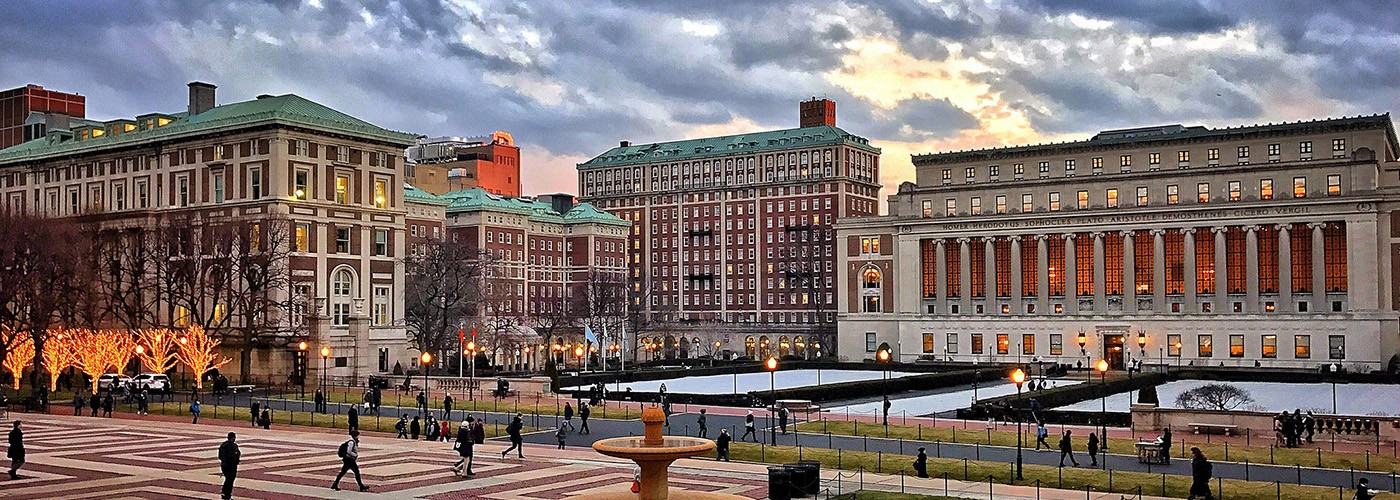
\includegraphics{cu.jpeg}
\caption{Test Photo}
\end{figure}


\end{document}
